\section{Extension to Dense Prediction}
\label{sec:segmentation}

A natural concern for any PEFT benchmark is whether the observed ranking is task-specific. Our main results cover single-label (EuroSAT) and multi-label (BigEarthNet-S2) classification; this section tests whether the same ranking holds on a \emph{dense prediction} task, where the adapter must shape not only a pooled class-token feature but also the full spatial feature grid. We port the three primary PEFT configurations to semantic segmentation on LandCover.ai~\cite{boguszewski2021landcoverai} and hold all other training-side choices fixed.

\subsection{Setup}

LandCover.ai provides 6-class land-cover segmentation on high-resolution aerial RGB tiles. We keep the same Prithvi-100M backbone used throughout the paper, reuse the existing \texttt{zero\_pad} input adapter, and first attach a lightweight linear segmentation head that upsamples the final transformer feature grid to the input resolution. This design intentionally isolates PEFT effects, but the lightweight linear segmentation decoder may limit absolute mIoU relative to heavier task-specific decoders. We therefore add a decoder-capacity ablation that keeps the same backbone, input adapter, optimizer setting, and three seeds while replacing the linear head with a shallow convolutional decoder of width 128. The PEFT-isolated comparison contains 9 runs (3 methods $\times$ 1 decoder $\times$ 3 seeds), and the decoder ablation contains 18 runs (3 methods $\times$ 2 decoders $\times$ 3 seeds). Performance is reported as mean Intersection-over-Union (mIoU) over the six semantic classes.

\subsection{Results}

Table~\ref{tab:landcoverai-seg} reports the aggregated results; per-seed values appear in Appendix~\ref{app:per-seed}.

\begin{table}[h]
\centering
\small
\caption{LandCover.ai semantic segmentation. Mean $\pm$ std mIoU over three seeds.}
\label{tab:landcoverai-seg}
\begin{tabular}{lccc}
\toprule
Method & Trainable Params & mIoU & $\Delta$ vs.\ Linear Probe \\
\midrule
Linear Probe & 4{,}614       & 0.2510 $\pm$ 0.0003 & --- \\
LoRA (r=8)   & 152{,}070     & 0.2510 $\pm$ 0.0001 & $+0.000$ \\
Houlsby      & 1{,}194{,}246 & \textbf{0.6410 $\pm$ 0.0029} & $\mathbf{+0.390}$ \\
\bottomrule
\end{tabular}
\end{table}

\begin{figure}[h]
\centering
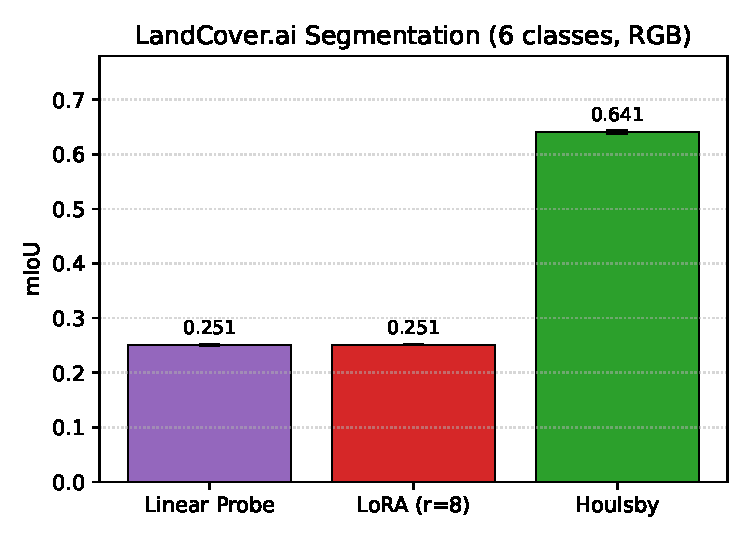
\includegraphics[width=0.62\linewidth]{figures/landcoverai_segmentation.pdf}
\caption{LandCover.ai mIoU by PEFT method (3 seeds each). Houlsby outperforms linear probing by $+155\%$ relative mIoU, while LoRA is statistically indistinguishable from linear probing to the fourth decimal place.}
\label{fig:seg-bars}
\end{figure}

We then tested whether the low absolute scores in Table~\ref{tab:landcoverai-seg} were caused by the adapter choice or by the segmentation decoder. Table~\ref{tab:landcoverai-decoder-ablation} reports the completed decoder-capacity ablation. Replacing the linear head with the convolutional decoder raises linear probing from 0.2509 to 0.6539 mIoU and LoRA from 0.2510 to 0.6547 mIoU. Houlsby also improves, from 0.6402 to 0.7246 mIoU, and remains the best method under the stronger decoder.

\begin{table}[h]
\centering
\small
\caption{LandCover.ai decoder-capacity ablation. Mean $\pm$ std mIoU over three seeds.}
\label{tab:landcoverai-decoder-ablation}
\begin{tabular}{llcc}
\toprule
Method & Decoder & Trainable Params & mIoU \\
\midrule
Linear Probe & Linear & 4{,}614 & 0.2509 $\pm$ 0.0003 \\
Linear Probe & Conv-lite ($d=128$) & 246{,}790 & 0.6539 $\pm$ 0.0021 \\
LoRA ($r=8$) & Linear & 152{,}070 & 0.2510 $\pm$ 0.0001 \\
LoRA ($r=8$) & Conv-lite ($d=128$) & 394{,}246 & 0.6547 $\pm$ 0.0041 \\
Houlsby & Linear & 1{,}194{,}246 & 0.6402 $\pm$ 0.0022 \\
Houlsby & Conv-lite ($d=128$) & 1{,}436{,}422 & \textbf{0.7246 $\pm$ 0.0028} \\
\bottomrule
\end{tabular}
\end{table}

Three observations carry over essentially unchanged from the classification results. First, Houlsby dominates by a large margin: $+0.390$ mIoU over linear probing, or a $+155\%$ relative gain. Second, LoRA offers no detectable improvement over linear probing; the two methods differ by less than $0.0001$ mIoU on each seed, with the LoRA standard deviation ($0.0001$) being even smaller than that of linear probing ($0.0003$). Third, the ordering Houlsby $\gg$ LoRA $\approx$ Linear~Probe is preserved across all three seeds without exception.

\subsection{Discussion}

The segmentation result is stronger than a consistency check. Relative to classification, the Houlsby--linear-probe gap widens from $+16.4\%$ OA on EuroSAT s2\_full to $+155\%$ mIoU on LandCover.ai under the PEFT-isolated linear decoder. Two mechanisms plausibly contribute. (i)~Dense prediction requires the adapter to shape every spatial token, not merely a pooled classifier input, so the per-layer bottleneck of a Houlsby adapter exerts influence at every position. (ii)~The linear-probe ceiling on LandCover.ai is low under the linear decoder (0.2510 mIoU), leaving more headroom for a capable adapter to exploit; this is the opposite regime from EuroSAT s2\_full, where linear probing already reaches 0.657 OA.

The decoder ablation confirms the setup warning: decoder capacity, not only PEFT capacity, strongly affects absolute LandCover.ai mIoU. With the conv-lite decoder, the best observed LandCover.ai result becomes 0.7246 $\pm$ 0.0028 mIoU for Houlsby, while linear probing and LoRA rise to 0.6539 and 0.6547 mIoU, respectively. The ordering still separates Houlsby from the linear-probe/LoRA cluster by about 0.070 mIoU under the stronger head, so the stronger decoder improves absolute performance without overturning the adapter-placement conclusion.

The LoRA result deserves explicit attention. On classification we reported that naive LoRA collapses to the linear-probe baseline within $\pm 0.001$ OA. Under the linear segmentation decoder the collapse is more extreme: the three LoRA seeds match the three linear-probe seeds to the fourth decimal place, indicating that the 152K LoRA parameters add no measurable dense-prediction benefit in this setting. The conv-lite ablation does not reverse this pattern, because LoRA remains within 0.001 mIoU of the frozen linear-probe baseline after both methods receive the stronger decoder. This is consistent with our classification-side diagnosis of a fused-QKV implementation trap compounded by a structural mismatch between low-rank adaptation and Prithvi-100M's pre-training regime; extending LoRA to dense prediction does not alter either cause.

Taken together, these experiments reduce the task-specificity concern but do not exhaust the segmentation design space. The PEFT ordering reported in the main benchmark, Houlsby $\gg$ LoRA $\approx$ Linear~Probe for the methods tested here, also appears under dense prediction with a larger Houlsby margin in the linear-decoder comparison and a smaller but persistent margin under the stronger conv-lite decoder. The ablation also narrows the earlier limitation: the linear decoder was indeed a major constraint on absolute LandCover.ai mIoU, but the paper still tests only one shallow convolutional decoder rather than the full range of task-specific segmentation heads.
